\begin{enumerate}[label=\thesubsection.\arabic*,ref=\thesubsection.\theenumi,itemsep=1ex]
%\numberwithin{equation}{enumi}
%
\item If $\cos x = -\frac{3}{5}, x$ lies in the third quadrant, find the values of other five trigonometric function.
%
\\
\solution
	In \figref{fig:ncert-id-1}, 
\begin{align}
	a &= -3, b = 5, c = -4
	\\
\implies \cos x &= -\frac{3}{5}\,
\sin x = -\frac{4}{5}\,
\tan x = \frac{-4}{-3}
\end{align}
\begin{figure}[H]
	\begin{center}
		{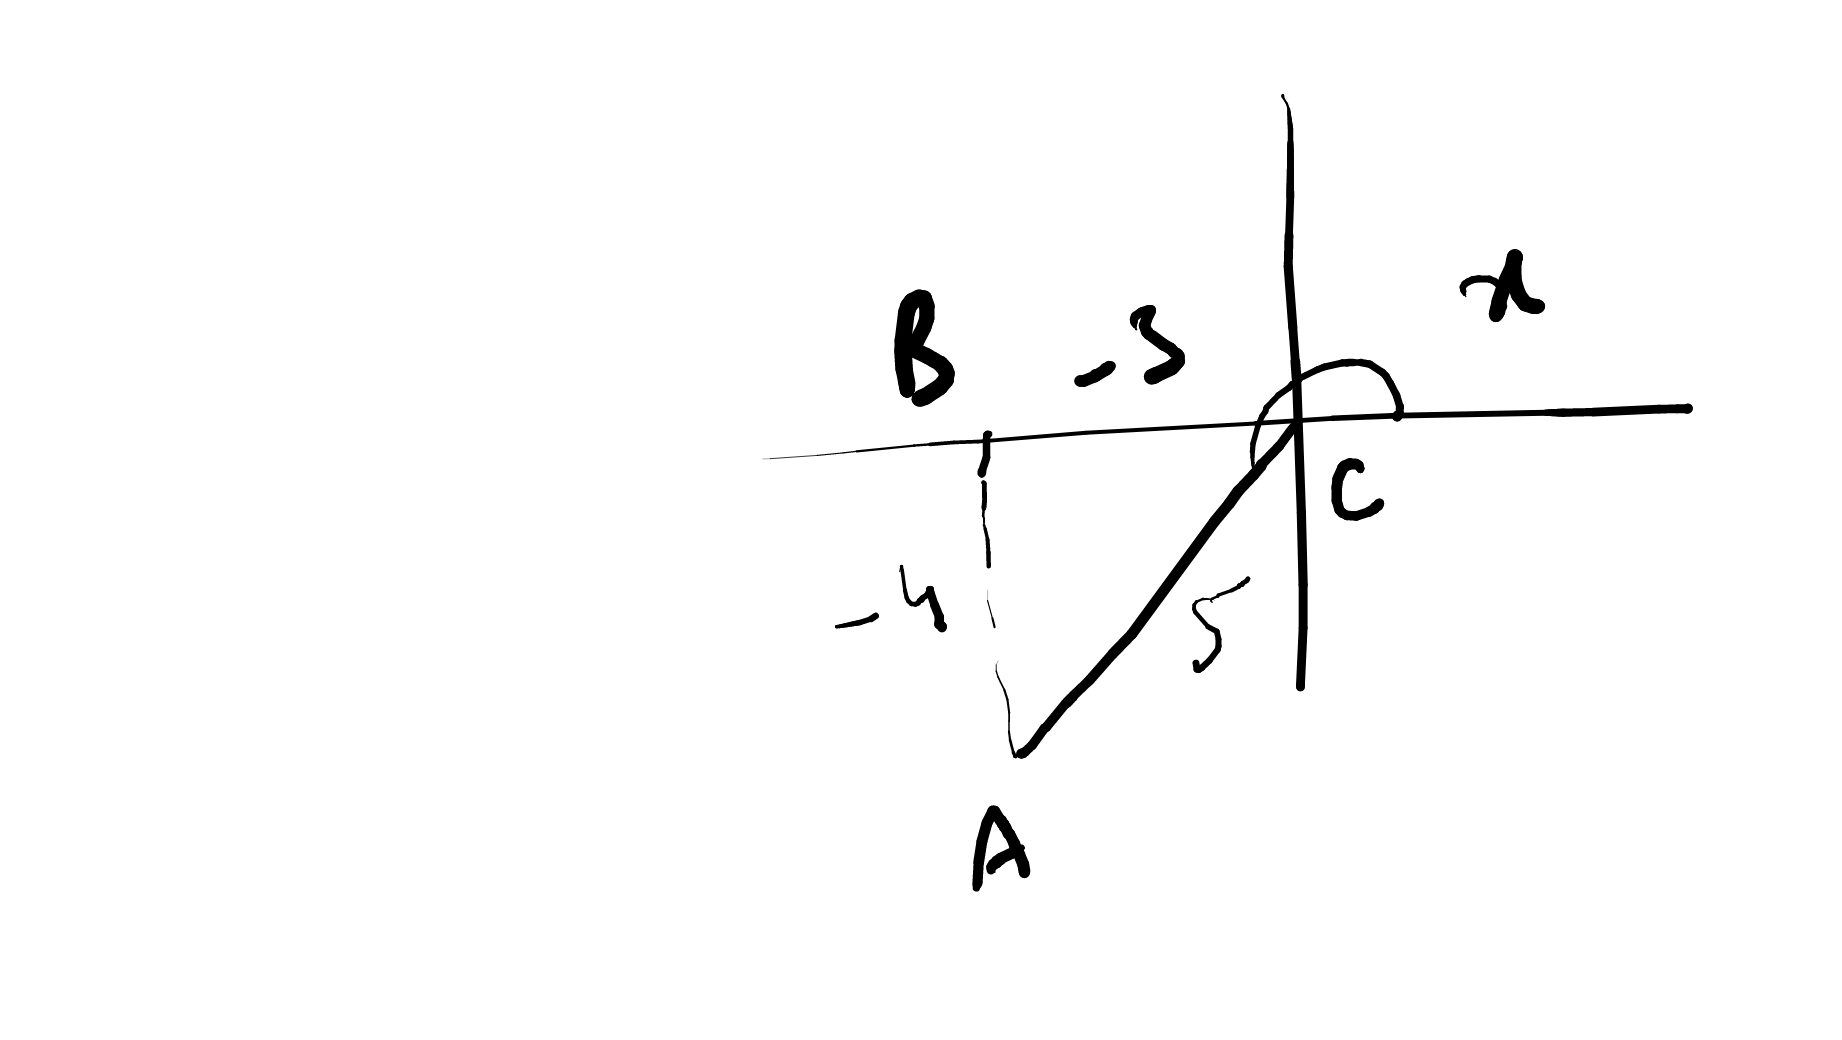
\includegraphics[width=0.6\columnwidth]{figs/ncert/id/1.png}}
	\end{center}
	\caption{}
	\label{fig:ncert-id-1}	
\end{figure}
\item If $\cot x = - \frac{5}{12}, x$ lies in the second quadrant, find the values of other five trigonometric function.
%
\\
\solution
	In \figref{fig:ncert-id-2}, 
\begin{align}
	a &= -5, b = 13, c = 12 
	\\
\implies \cos x &= -\frac{5}{13}\,
\sin x = \frac{12}{13}\,
\tan x = -\frac{12}{5}
\end{align}
\begin{figure}[H]
	\begin{center}
		{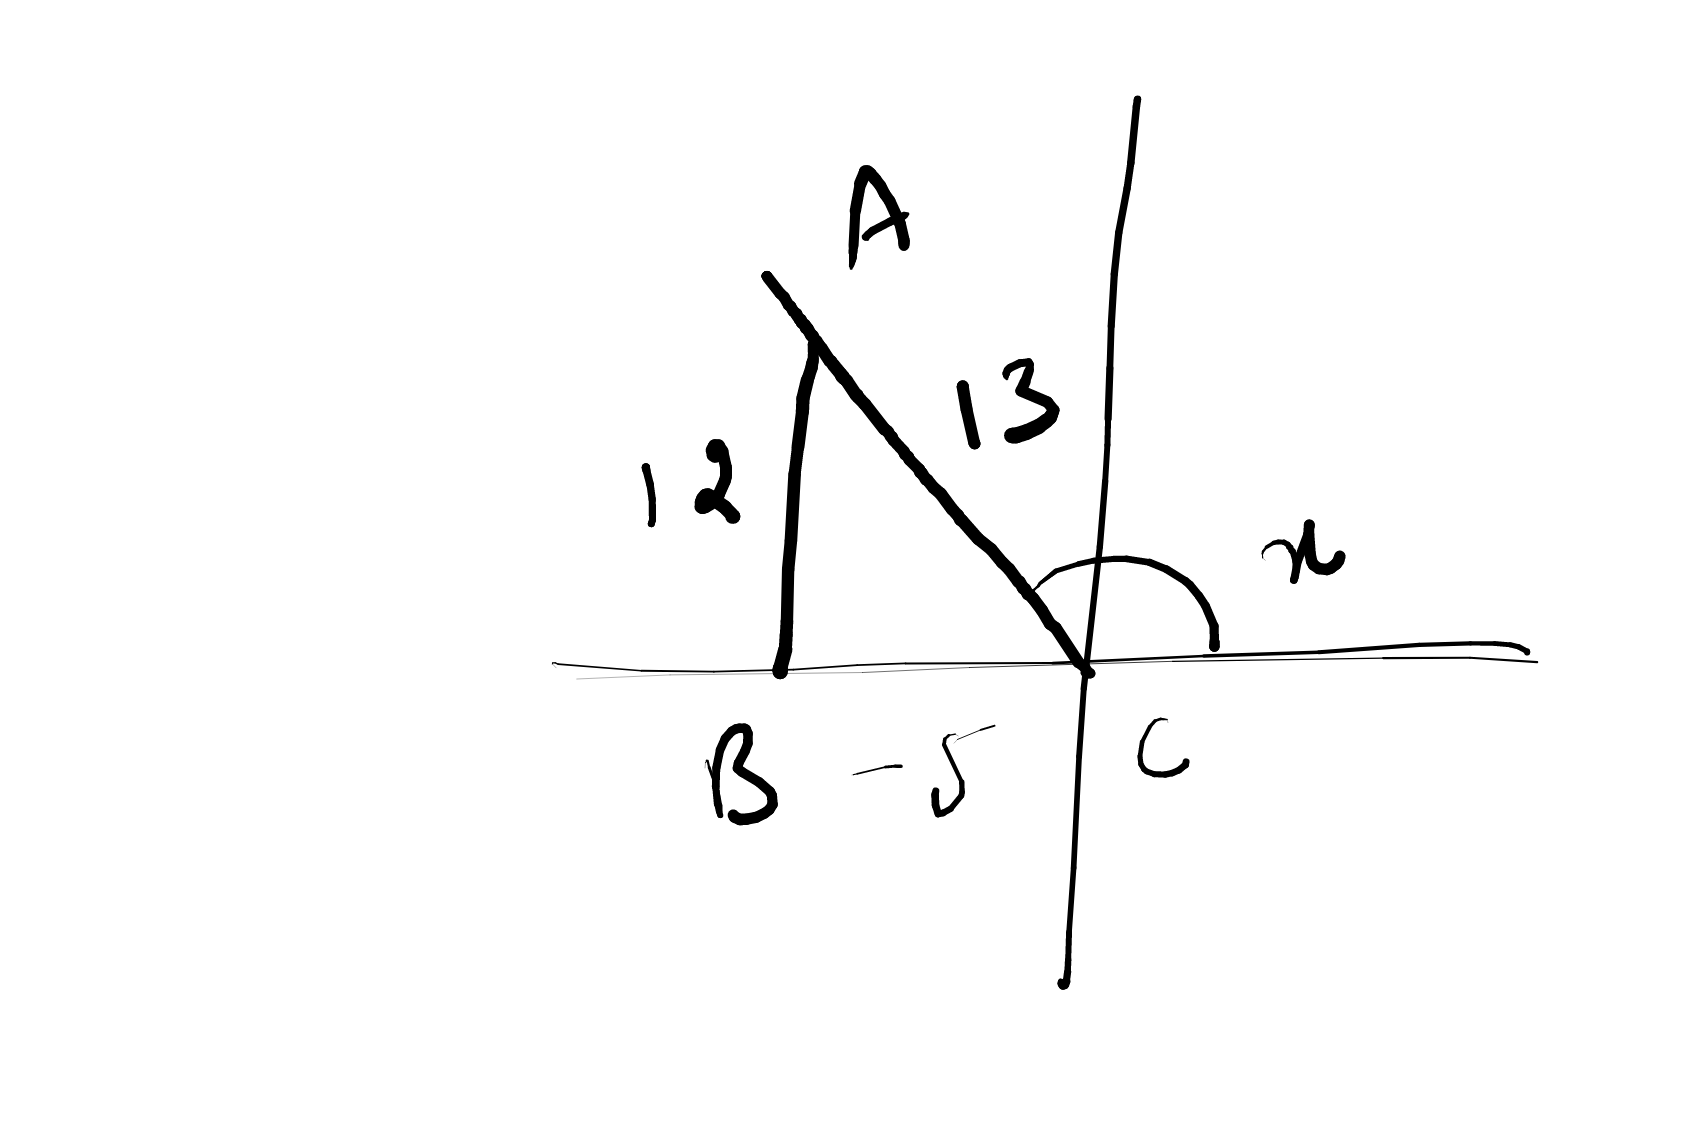
\includegraphics[width=0.6\columnwidth]{figs/ncert/id/2.png}}
	\end{center}
	\caption{}
	\label{fig:ncert-id-2}	
\end{figure}
\item Find the value of $\sin \frac{31\pi}{3}$.
%
	\\
		\solution 
\begin{align}
	\sin \frac{31\pi}{3} &= 
	\sin \brak{10 \pi+\frac{\pi}{3}} 
	\\
	&= 
	\sin \brak{\frac{\pi}{3}} = \frac{1}{2}
\end{align}
\item Find the value of $\cos\brak{-1710\degree}$.
%
	\\
		\solution 
\begin{align}
	\cos\brak{-1710\degree}	&= 
\cos\brak{-5\times360\degree+90\degree}	 
\\
	&=\cos{90\degree}	= 0
\end{align}
\item Prove that $3\sin\frac{\pi}{6}\sec\frac{\pi}{3}-4\sin\frac{5\pi}{6}\cot\frac{\pi}{4} = 1.$
%
	\\
	\solution
\begin{align}
	3\sin\frac{\pi}{6}\sec\frac{\pi}{3}-4\sin\frac{5\pi}{6}\cot\frac{\pi}{4} &= 
	3\frac{\sin\frac{\pi}{6}}{\cos\brak{\frac{\pi}{2}-\frac{\pi}{6}}}-4\sin\brak{\pi - \frac{\pi}{6}}  
	\\
	&=
	3\frac{\sin\frac{\pi}{6}}{\sin\frac{\pi}{6}}-4\sin\brak{ \frac{\pi}{6}}  
	= 1
\end{align}
upon substituting numerical values.
\item Find the value of $\sin 15\degree$.
%
	\\
	\solution 
\begin{align}
	1 - 2 \sin^2 15 &= \cos 30 = \frac{\sqrt{3}}{2}
	\\
	\implies 
	\sin 15 &= \sqrt{\frac{1-\frac{\sqrt{3}}{2}}{2}}
	 = \frac{\sqrt{2-\sqrt{3}}}{2}
	 \label{eq:id-sin15}
\end{align}
\item Find the value of $\tan\frac{13\pi}{12}$.
%
	\\
	\solution 
\begin{align}
\tan\frac{13\pi}{12}
	&=
	\tan\brak{\pi+\frac{\pi}{12}}
=\tan\frac{\pi}{12}
\end{align}
%
Since
\begin{align}
	2 \cos^2 15 -1 &= \cos 30 = \frac{\sqrt{3}}{2},
	\\
	\cos15 &= \sqrt{\frac{1+\frac{\sqrt{3}}{2}}{2}}
	 = \frac{\sqrt{2+\sqrt{3}}}{2}
	 \label{eq:id-cos15}
	 \\
	 \therefore 
	\tan\frac{\pi}{12} &= \frac{\sin 15}{\cos15}
	 = \frac{\sqrt{2-\sqrt{3}}}{\sqrt{2+\sqrt{3}}}
	 \label{eq:id-tan15}
\end{align}
upon substituting from 
	 \eqref{eq:id-sin15}.
\item Prove that 
\begin{align}
	\frac{\sin\brak{x+y}}{\sin\brak{x-y}} = \frac{\tan x + \tan y}{\tan x - \tan y}.
	 \label{eq:id-cosxcosy}
\end{align}
%
	\\
	\solution
\begin{align}
\frac{\sin\brak{x+y}}{\sin\brak{x-y}} = \frac{\sin x \cos y +\sin y \cos x }{\sin x \cos y -\sin y \cos x }
\end{align}
Dividing the numerator and denominator by $\cos x \cos y$
%
yields
	 \eqref{eq:id-cosxcosy}.
\item Show that
\begin{align}
	 \label{eq:id-tanx2x3x}
\tan3x\tan2x\tan x = \tan3x-\tan2x-\tan x
\end{align}
%
\\
\solution
\begin{align}
	\tan3x = \tan \brak{2x +\tan x} &= \frac{\tan 2x + \tan x}{1 - \tan x \tan 2x}
	\\
	\implies 
	\tan3x \brak{1 - \tan x \tan 2x}&= {\tan 2x + \tan x}
\end{align}
%
yielding
	 \eqref{eq:id-tanx2x3x}.
\item Prove that
\begin{align}
\cos\brak{\frac{\pi}{4}+x} + \cos\brak{\frac{\pi}{4}-x} = \sqrt 2\cos x.
	 \label{eq:id-sqrt2cosx}
\end{align}
%
\\
\solution
\begin{align}
\cos\brak{\frac{\pi}{4}+x} + \cos\brak{\frac{\pi}{4}-x} = 
2\cos\brak{\frac{\pi}{4}} \cos x  
\end{align}
yielding
	 \eqref{eq:id-sqrt2cosx}
	 after substituting numerical values.
%
\item Prove that 
%
\begin{align}
\frac{\cos7x+\cos5x}{\sin7x-\sin 5x} 
=\cot x
	 \label{eq:id-cotx}
\end{align}
%
\\
\solution
\begin{align}
\frac{\cos7x+\cos5x}{\sin7x-\sin 5x} 
=\frac{2\cos6x\cos x}{2\cos 6x\cos x} 
\end{align}
yielding
	 \eqref{eq:id-cotx}.
\item Prove that 
\begin{align}
	\frac{\sin5x-2\sin3x+\sin x}{\cos5x-\cos x} = \tan x.
	 \label{eq:id-tanx}
\end{align}
%
\\
\solution
\begin{align}
	\frac{\sin5x-2\sin3x+\sin x}{\cos5x-\cos x} 
	&=
	-\frac{2\sin3x\cos2x-2\sin3x}{2\sin 3x\sin 2x}
	\\
	&=
	\frac{1-\cos2x}{\sin2x} = \frac{2\sin^2 x}{2\sin x\cos x}
\end{align}
	 yielding \eqref{eq:id-tanx}.
%
\item If $\sin x=\frac{3}{5}, \cos y=-\frac{12}{13}$, where $x$ and $y$
both lies in second quadrant, find the value of
$\sin\brak{x+y}$.
%
\\
\solution 
From the given information,
\begin{align}
	\cos x &= -\frac{4}{5},
	\sin y = \frac{5}{13}
	\\
	\implies 
	\sin\brak{x+y} &= -\frac{3}{5}\times \frac{12}{13} - \frac{4}{5}\times \frac{5}{13}
	\\
	&=-\frac{56}{65}
\end{align}
%
\item Prove that
\begin{align}
\cos2x\cos\frac{x}{2}-\cos3x\cos\frac{9x}{2}=\sin5x\sin\frac{5x}{2}.
	 \label{eq:id-sin5x}.
\end{align}
%
\\
\solution 
\begin{align}
\cos2x\cos\frac{x}{2}
	&=\frac{1}{2}\brak{\cos\brak{2x+\frac{x}{2}}+\cos\brak{2x-\frac{x}{2}}}
	\\
\cos3x\cos\frac{9x}{2}
	&=\frac{1}{2}\brak{\cos\brak{3x+\frac{9x}{2}}+\cos\brak{3x-\frac{9x}{2}}}
\end{align}
Also,
\begin{align}
	\cos\brak{2x+\frac{x}{2}}-
\cos\brak{3x+\frac{9x}{2}}
	&= 2\sin 5x \sin \frac{5x}{2}
\\
\cos\brak{2x-\frac{x}{2}}
-
\cos\brak{3x-\frac{9x}{2}}
	&= 0
\end{align}
%
yielding
	 \eqref{eq:id-sin5x} after some algebra.
\item Find the value of $\tan\frac{\pi}{8}$.
%
	\\
	\solution
\begin{align}
	\tan 2\theta = \frac{2\tan \theta}{1-\tan^2\theta}
\label{eq:id-tantheta}
\end{align}
For $\theta = \frac{\pi}{8}$,  we obtain
\begin{align}
	 \frac{2\tan \theta}{1-\tan^2\theta}=1
	 \implies 
	{\tan^2\theta}+{2\tan \theta}- 1=0
\end{align}
yielding
\begin{align}
	\tan \theta = \sqrt{2}-1 
\end{align}
by taking the positive root of the quadratic.
%
\item If $\tan x=\frac{3}{4}, \pi<x<\frac{3\pi}{2}$, find the value of $\sin\frac{x}{2},\cos\frac{x}{2}$ and $\tan\frac{x}{2}$.
%
	\\
	\solution $ \frac{\pi}{2}<\frac{x}{2} <\frac{3\pi}{4} $, hence $\frac{x}{2}$
	lies in the $2^{nd}$
	quadrant.
%
	For $\theta = \frac{x}{2}$
	in
\eqref{eq:id-tantheta},
\begin{align}
	3{\tan^2\theta}+{8\tan \theta}- {3}=0
	\\
	\implies
	\tan\frac{x}{2}=\tan \theta = -3
\end{align}
by taking the negative root.
From
	\figref{fig:ncert-id-3},	
\begin{align}
	\cos \frac{x}{2} = -\frac{1}{\sqrt{10}},
	\sin\frac{x}{2} = \frac{3}{\sqrt{10}}
\end{align}
\begin{figure}[H]
	\begin{center}
		{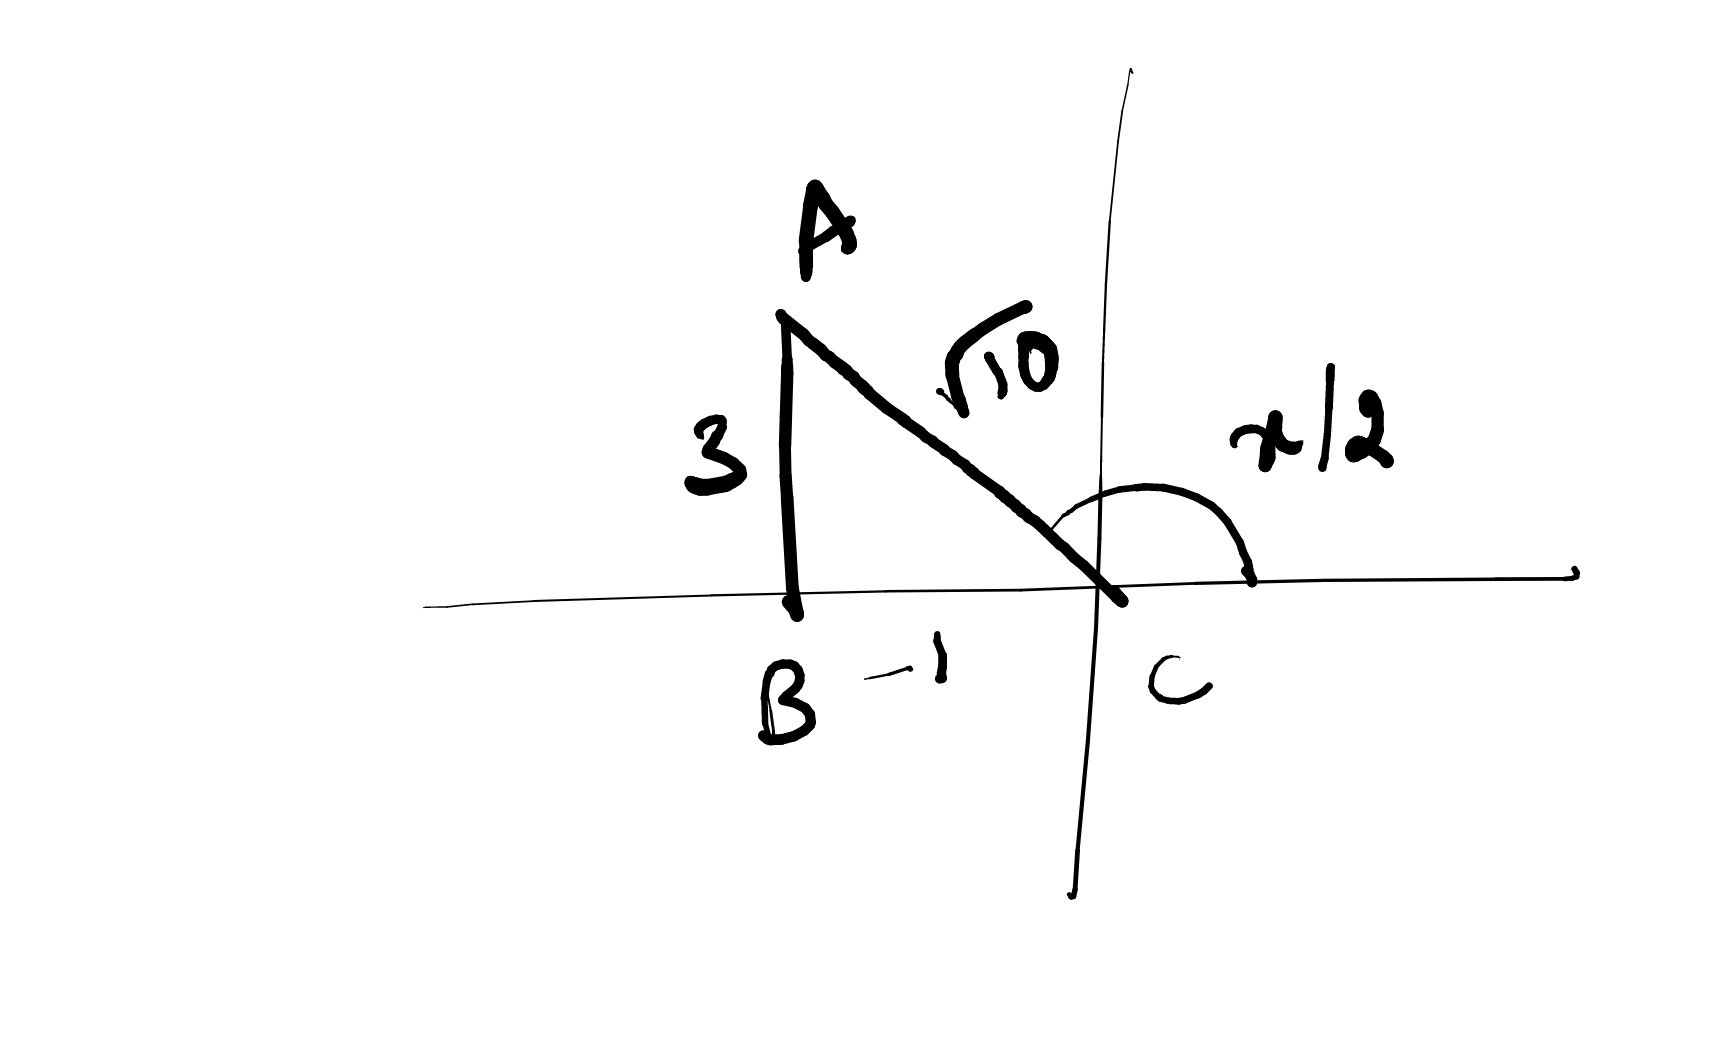
\includegraphics[width=0.6\columnwidth]{figs/ncert/id/3.png}}
	\end{center}
	\caption{}
	\label{fig:ncert-id-3}	
\end{figure}
\item Prove that
$\cos^{2}x+\cos^{2}\brak{x+\frac{\pi}{3}}+\cos^{2}\brak{x-\frac{\pi}{3}}=\frac{3}{2}$.
%
\\
\solution The LHS can be expressed as
\begin{multline}
	\frac{1 + \cos 2x + 1 + \cos\brak{2x+\frac{2\pi}{3}}+ 1+\cos\brak{2x-\frac{2\pi}{3}}}{2}
	\\
	=
	\frac{3}{2} +
	\frac{\cos 2x + 2\cos2x\cos \brak{\frac{2\pi}{3}}}{2}
\end{multline}
yielding the RHS upon substituting numerical values.
\item Find the values of other five trigonometric functions 
\begin{enumerate}
	\item $\cos x=-\frac{1}{2}$, $x$  lies in third quadrant.
	\item $\sin x= \frac{3}{5} $,$ x$  lies in second quadrant.
	\item $\cot x= \frac{3}{4}$,$ x$  lies in third quadrant.
	\item $\sec x= \frac{13}{5}$, $x$  lies in fourth quadrant.
	\item $\tan x=-\frac{5}{12}$, $x$  lies in second quadrant.
\end{enumerate}
%
\solution
\begin{enumerate}
	\item 
	See \figref{fig:ncert-id-4}.	
\begin{align}
	\sin x = -\frac{\sqrt{3}}{2},
	\tan x = {\sqrt{3}}
\end{align}
\begin{figure}[H]
	\begin{center}
		{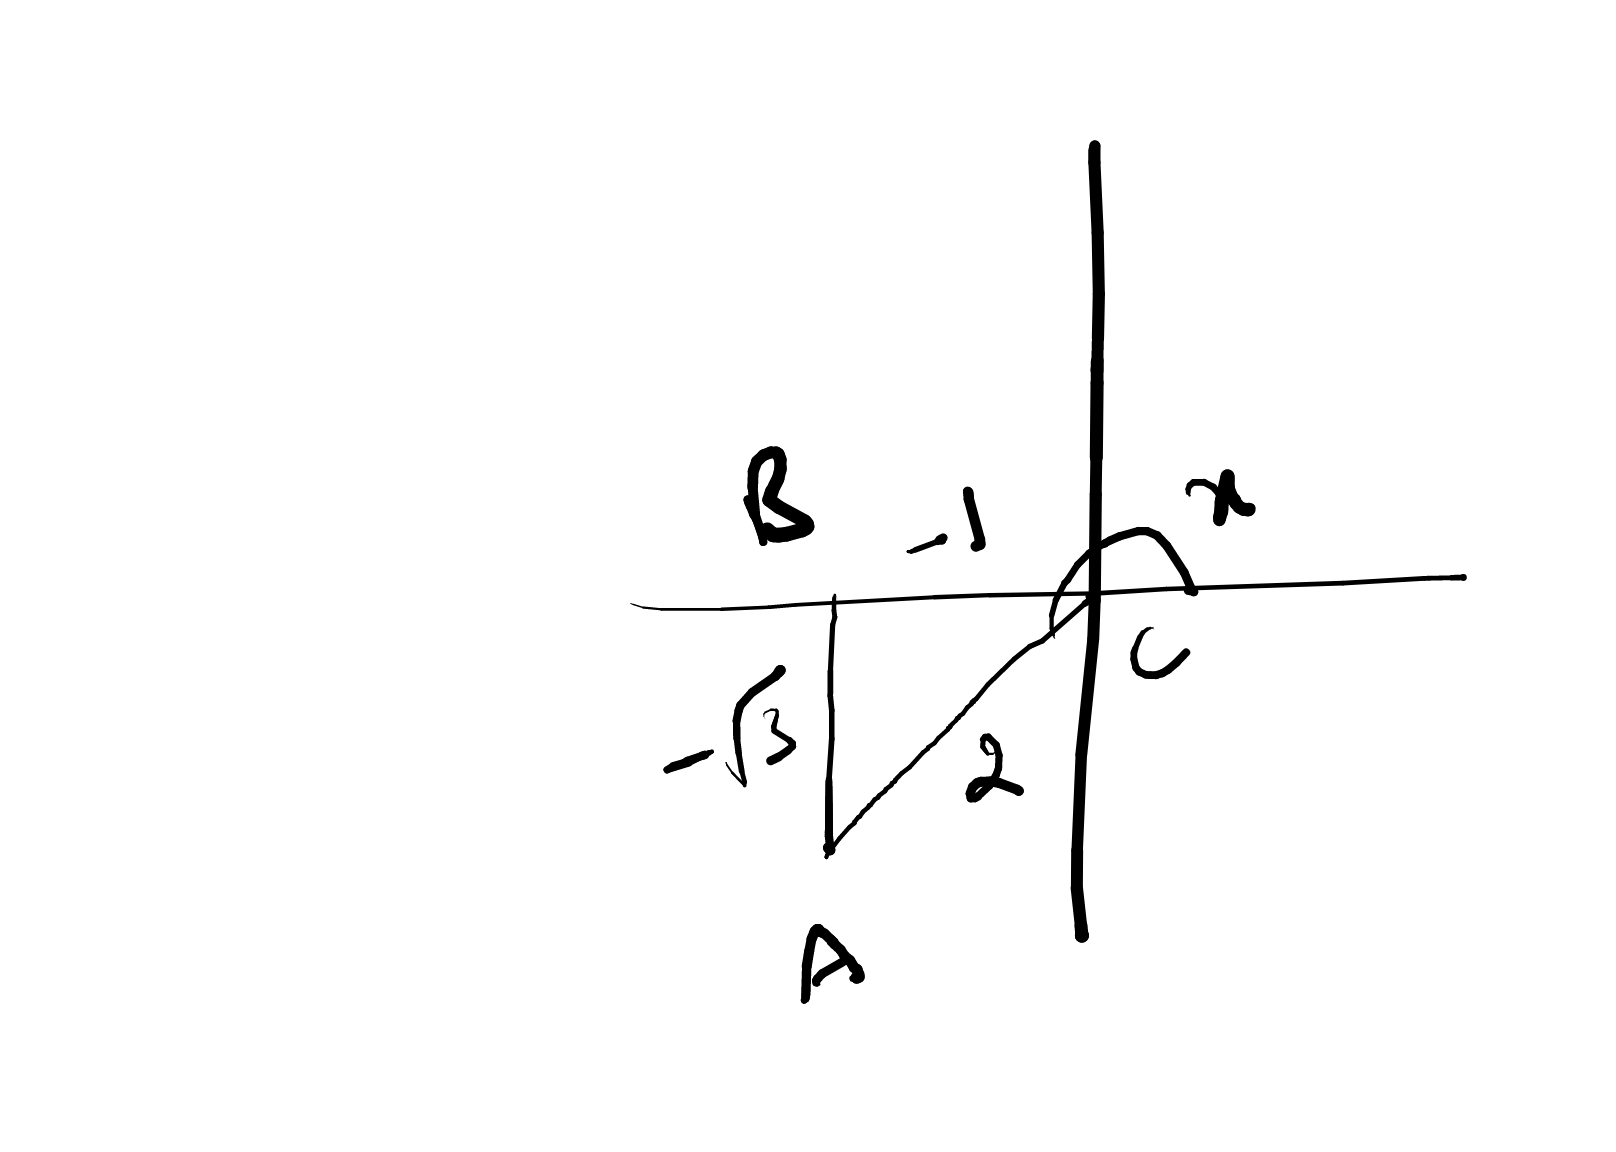
\includegraphics[width=0.6\columnwidth]{figs/ncert/id/4.png}}
	\end{center}
	\caption{}
	\label{fig:ncert-id-4}	
\end{figure}
	\item 
	See \figref{fig:ncert-id-5}.	
\begin{align}
	\cos x = -\frac{4}{5},
	\tan x = -\frac{3}{4}.
\end{align}
\begin{figure}[H]
	\begin{center}
		{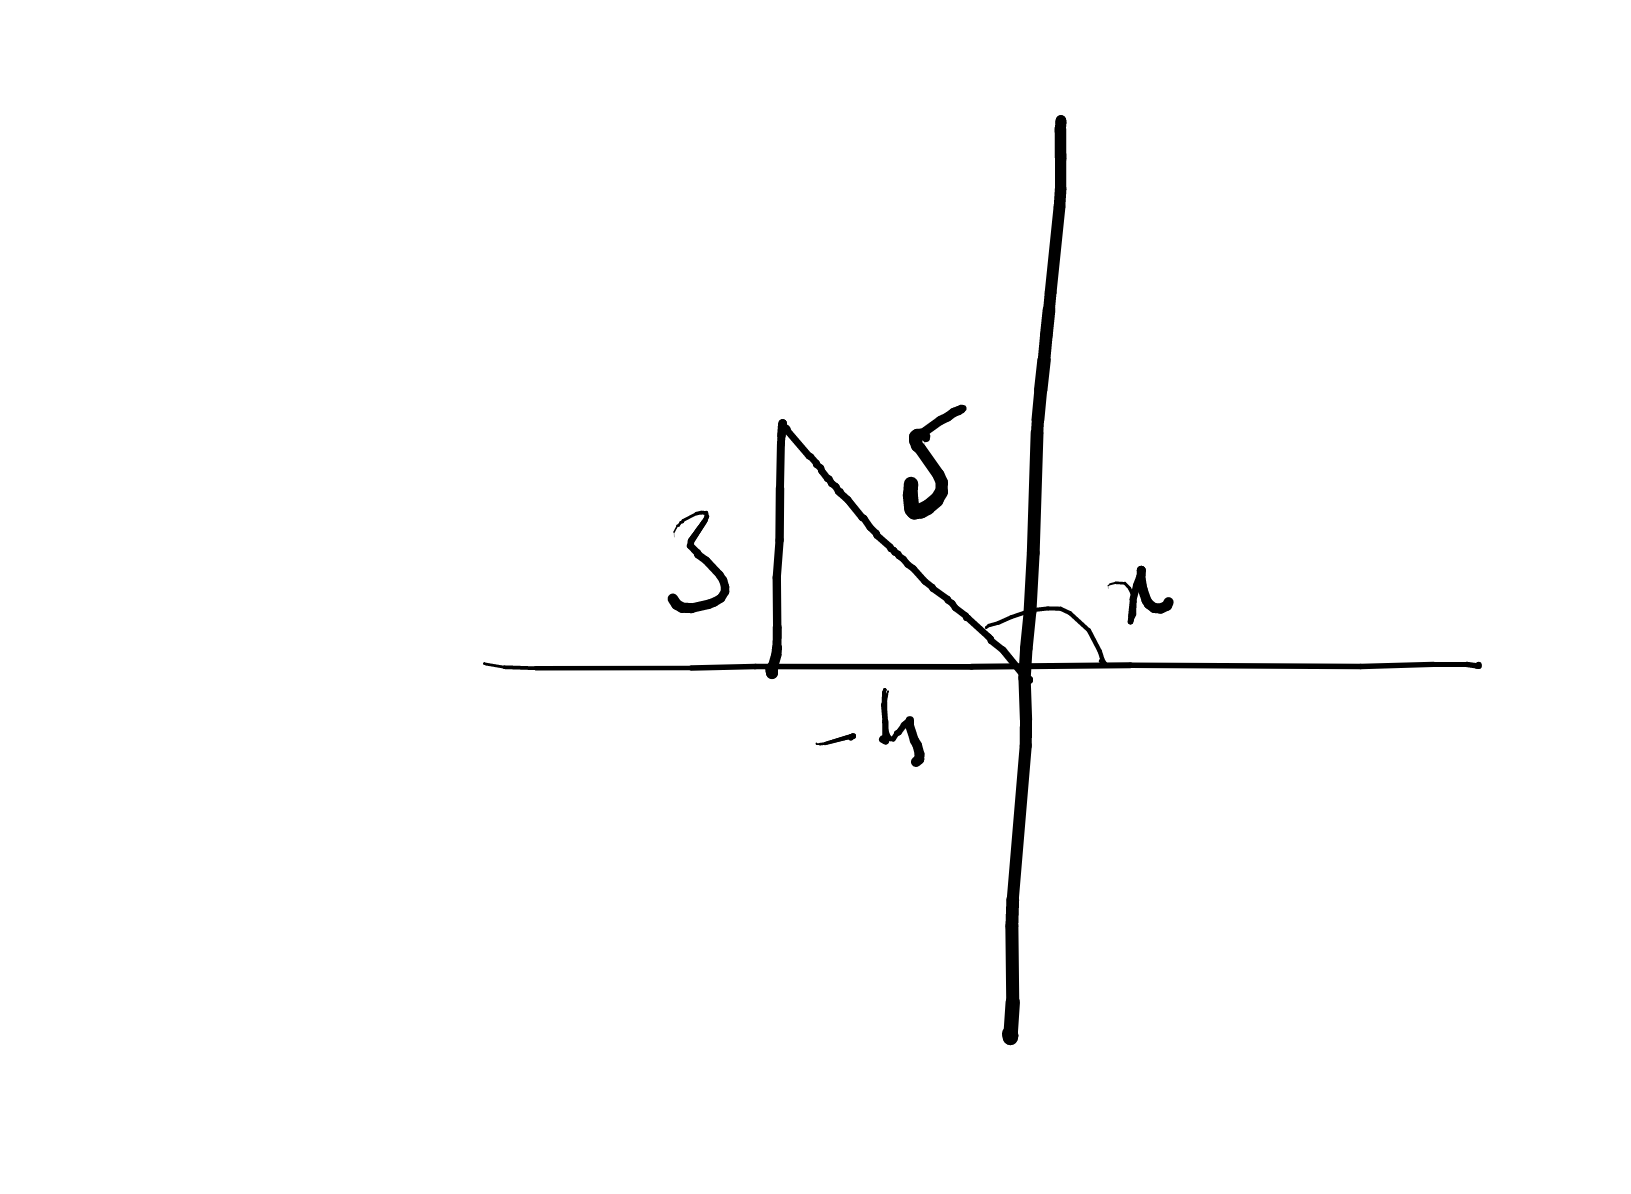
\includegraphics[width=0.6\columnwidth]{figs/ncert/id/5.png}}
	\end{center}
	\caption{}
	\label{fig:ncert-id-5}	
\end{figure}
	\item 
	See \figref{fig:ncert-id-6}.
\begin{align}
	\cos x = -\frac{3}{5},
	\sin x = -\frac{4}{5},
	\tan x = \frac{4}{3}.
\end{align}
\begin{figure}[H]
	\begin{center}
		{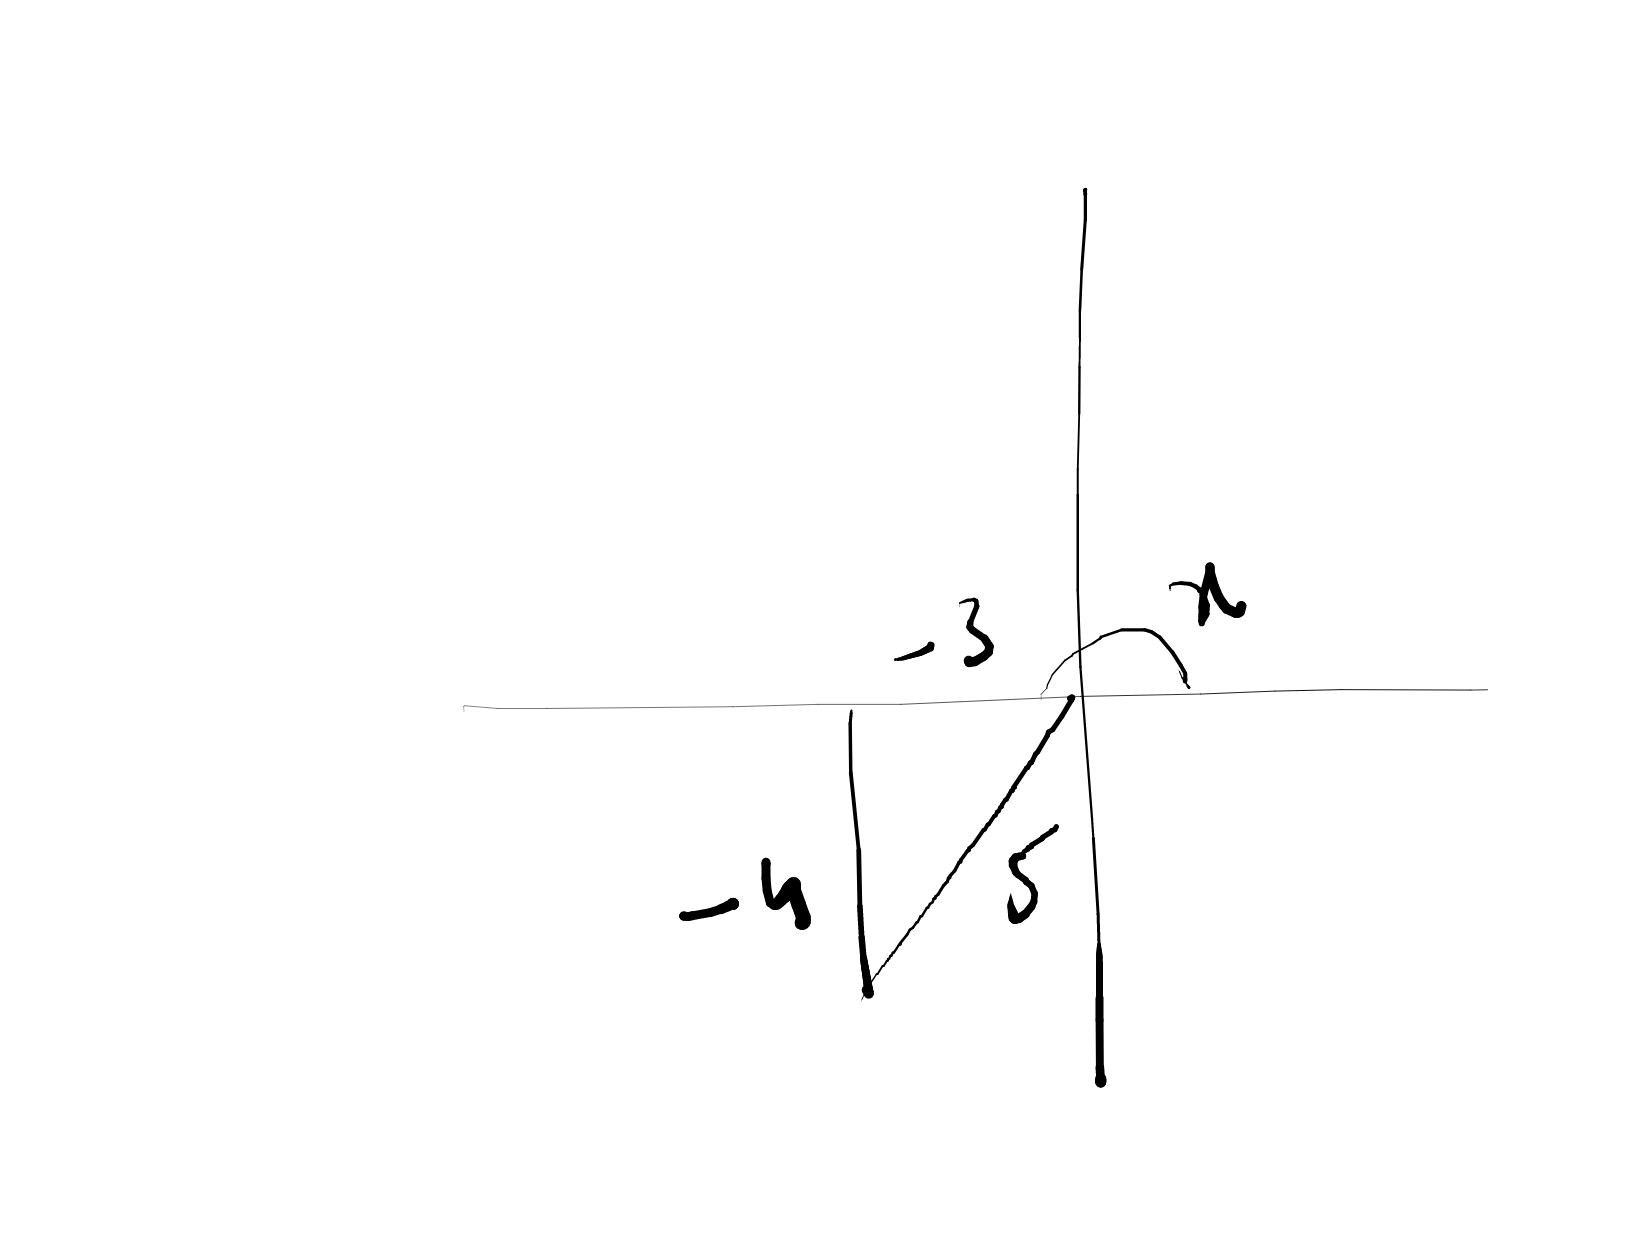
\includegraphics[width=0.6\columnwidth]{figs/ncert/id/6.png}}
	\end{center}
	\caption{}
	\label{fig:ncert-id-6}	
\end{figure}
	\item 
	See \figref{fig:ncert-id-7}.	
\begin{align}
	\cos x = \frac{5}{13},
	\sin x = -\frac{12}{13},
	\tan x = -\frac{12}{5}.
\end{align}
\begin{figure}[H]
	\begin{center}
		{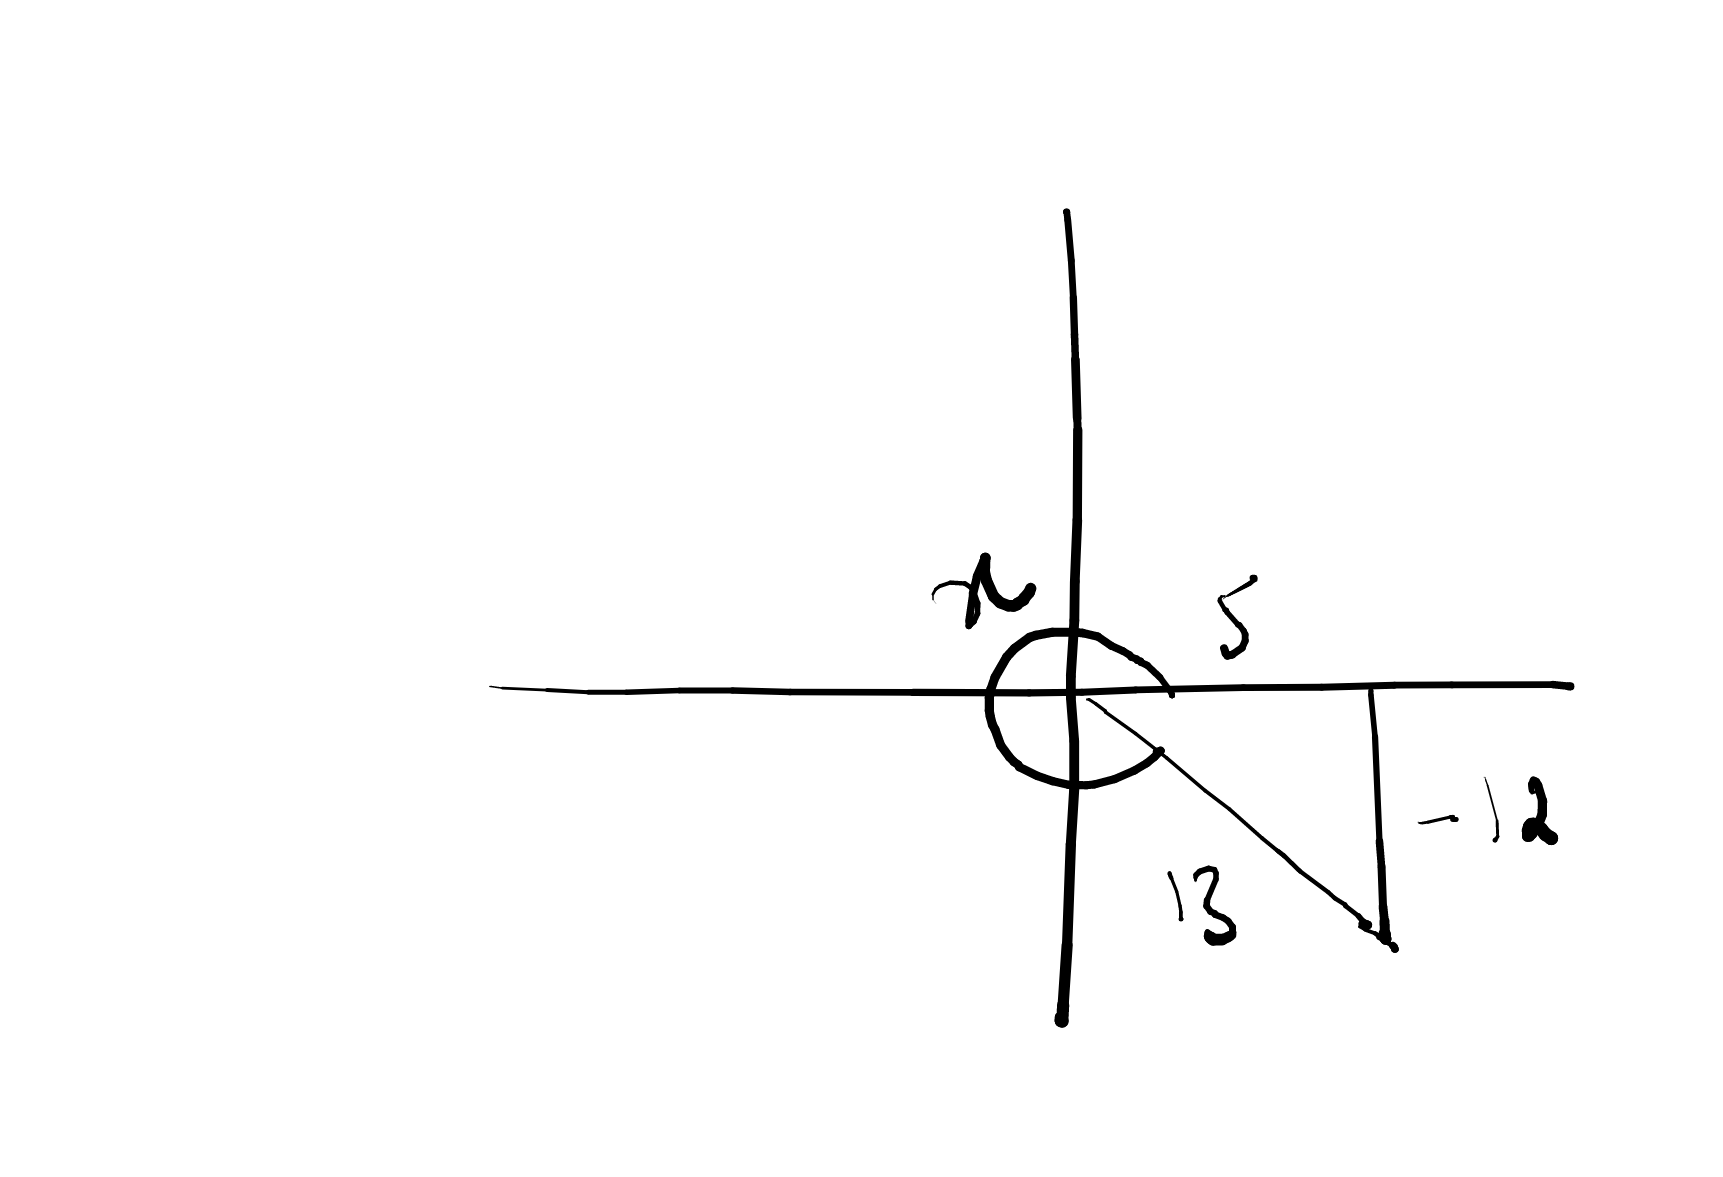
\includegraphics[width=0.6\columnwidth]{figs/ncert/id/7.png}}
	\end{center}
	\caption{}
	\label{fig:ncert-id-7}	
\end{figure}
	\item 
	See \figref{fig:ncert-id-8}.	
\begin{align}
	\cos x = -\frac{12}{13},
	\sin x = \frac{5}{13}
\end{align}
\begin{figure}[H]
	\begin{center}
		{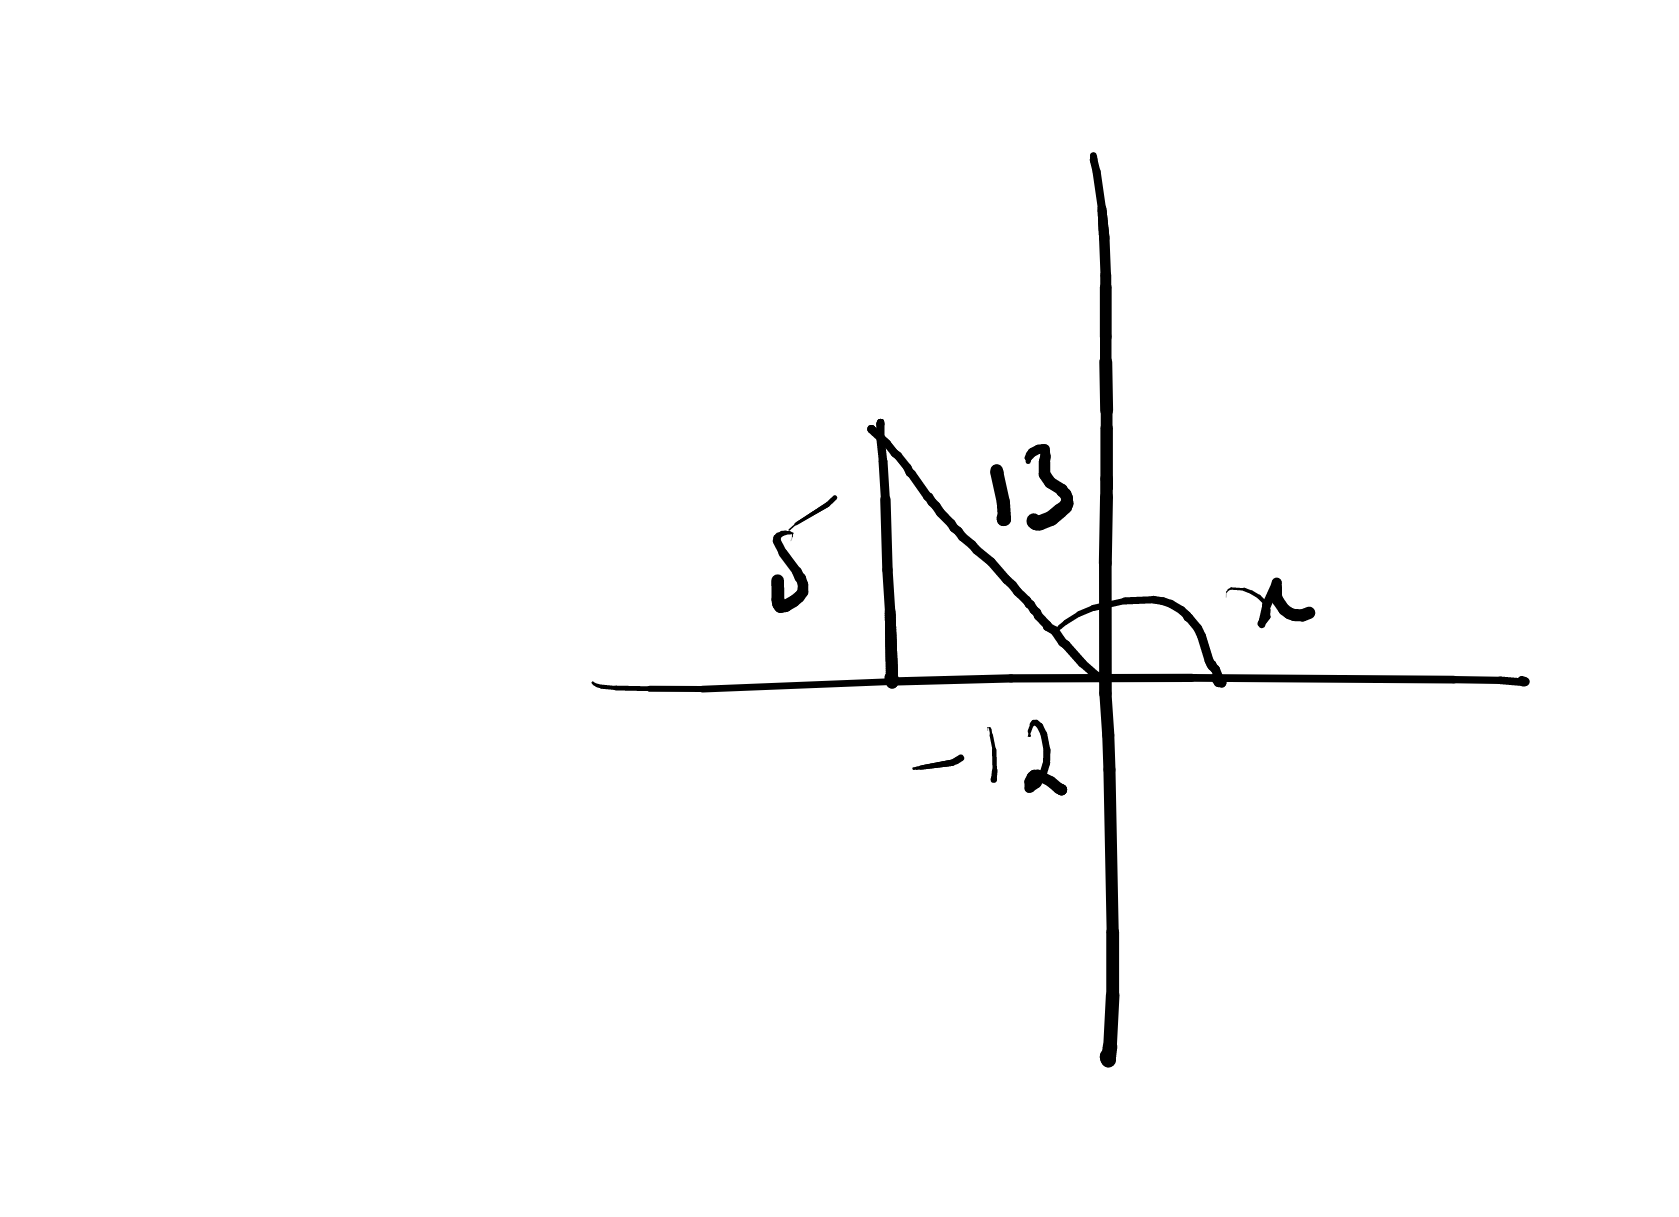
\includegraphics[width=0.6\columnwidth]{figs/ncert/id/8.png}}
	\end{center}
	\caption{}
	\label{fig:ncert-id-8}	
\end{figure}
\end{enumerate}
\item Find the values of the trigonometric functions
\begin{multicols}{2}
\begin{enumerate}
\item $\sin765\degree$
\item $\csc\brak{-1410\degree}$
\item $\tan\frac{19\pi}{3}$
\item $\sin\frac{-11\pi}{3}$
\item $\cot\frac{-15\pi}{4}$
\end{enumerate}
\end{multicols}
%
\solution
\begin{enumerate}
\item 
\begin{align}
	\sin765\degree &= \sin \brak{2\times 360\degree + 45 \degree}
	\\
	&= \sin 45\degree = \frac{1}{\sqrt{2}}
\end{align}
\item 
\begin{align}
	\csc\brak{-1410\degree}&=	
\csc\brak{-4\times 360\degree + 30 \degree}
\\
	&= \csc 30 \degree = {2}
\end{align}
\item 
\begin{align}
\tan\frac{19\pi}{3}
	&=	
	\tan\brak{6\pi + \frac{\pi}{3}}
	\\
	&= \tan \frac{\pi}{3}= {\sqrt{3}}
\end{align}
\item 
\begin{align}
\sin\frac{-11\pi}{3}
	&=\sin\brak{-4\pi +\frac{\pi}{3}}
	\\
	&=\sin{\frac{\pi}{3}}=\frac{\sqrt{3}}{2}
\end{align}
\item $\cot\frac{-15\pi}{4}$
\begin{align}
\cot\frac{-15\pi}{4}
	&=\cot\brak{-4\pi+\frac{\pi}{4}}
	\\
	&=\cot{\frac{\pi}{4}}=1
\end{align}
\end{enumerate}
\item Prove that
\begin{multicols}{2}
\begin{enumerate}
\item $\sin^{2}\frac{\pi}{6}+\cos^{2}\frac{\pi}{3}-\tan^{2}\frac{\pi}{4}=-\frac{1}{2}$
\item $2\sin^{2}\frac{\pi}{6}+\csc^{2}\frac{7\pi}{6}\cos^{2}\frac{\pi}{3}=\frac{3}{2}$
\item $\cot^{2}\frac{\pi}{6}+\csc\frac{5\pi}{6}+3\tan^{2}\frac{\pi}{6}$=6
\item $2\sin^{2}\frac{3\pi}{4}+2\cos^{2}\frac{\pi}{4}+2\sec^{2}\frac{\pi}{3}$=10
\end{enumerate}
\end{multicols}
%
\solution
\begin{enumerate}
\item The LHS is
\begin{align}
\sin^{2}\frac{\pi}{6}+\sin^{2}\frac{\pi}{6}-1
	&=
\sin^{2}\frac{\pi}{6}-\cos^{2}\frac{\pi}{6}
\\
	&=-\cos\frac{\pi}{3}=-\frac{1}{2}
\end{align}
\item The LHS can be expressed as
\begin{align}
	2\sin^{2}\frac{\pi}{6}+\frac{\cos^{2}\frac{\pi}{3}}{\sin^{2}\brak{\pi +\frac{\pi}{6}}} &= 
	2\sin^{2}\frac{\pi}{6}+\frac{\sin^{2}\frac{\pi}{6}}{\sin^{2}{\frac{\pi}{6}}} = \frac{1}{2} + 1 
\end{align}
\item The LHS equals
\begin{align}
	\tan^{2}\frac{\pi}{6}+\cot^{2}\frac{\pi}{6}+\csc\brak{\pi-\frac{\pi}{6}}+2\tan^{2}\frac{\pi}{6}
	&=
	\brak{\tan\frac{\pi}{6}+\cot\frac{\pi}{6}}^2-2+\csc{\frac{\pi}{6}}+2\tan^{2}\frac{\pi}{6}
	\\
	&=
	\sec^2\frac{\pi}{6}\csc^2\frac{\pi}{6}-2+2+2\tan^{2}\frac{\pi}{6}
	\\
	&=
	4\sec^2\frac{\pi}{6}+2\tan^{2}\frac{\pi}{6}
	\\
	&=
	4+6\tan^2\frac{\pi}{6} = 6
\end{align}
\item The LHS can be expressed as
\begin{align}
	2\sin^{2}\brak{\pi -\frac{\pi}{4}}+2\cos^{2}\frac{\pi}{4}+2\sec^{2}\frac{\pi}{3} &= 
	2\brak{\sin^{2}\frac{\pi}{4}+\cos^{2}\frac{\pi}{4}}+8
\end{align}
\end{enumerate}
\item Find the value of
\begin{multicols}{2}
\begin{enumerate}
\item$\sin75\degree$
\item $\tan15\degree$
\end{enumerate}
\end{multicols}
%
\solution
\begin{enumerate}
\item 
\begin{align}
\sin 75\degree 
=\cos 15\degree 
\end{align}
	 which is available in \eqref{eq:id-cos15}.
\item See
	 \eqref{eq:id-tan15}.
\end{enumerate}
\item Prove that 
 $\cos\brak{\frac{\pi}{4}-x}\cos\brak{\frac{\pi}{4}-y}-\sin\brak{\frac{\pi}{4}-x}\sin\brak{\frac{\pi}{4}-y}=\sin\brak{x+y}$.
%
 \\
 \solution
 The LHS can be expressed as
\begin{align}
	\cos\brak{\frac{\pi}{4}-x+\frac{\pi}{4}-y}&=\cos\sbrak{\frac{\pi}{2}-\brak{x+y}}
\end{align}
which is equal to the RHS.
\item Prove that 
$$\frac{\tan\brak{\frac{\pi}{4}+x}}{\tan\brak{\frac{\pi}{4}-x}}=\brak{\frac{1+\tan x}{1-\tan x}}^{2}.$$
%
\solution
\begin{align}
	{\tan\brak{\frac{\pi}{4}+x}}&=\frac{\tan\frac{\pi}{4}+\tan x}{1-\tan\frac{\pi}{4}\tan x}
	\\
	&=\frac{1+\tan x}{1-\tan x}
	\\
{\tan\brak{\frac{\pi}{4}-x}}&=\frac{\tan\frac{\pi}{4}-\tan x}{1+\tan\frac{\pi}{4}\tan x}
	\\
	&=\frac{1-\tan x}{1+\tan x}
\end{align}
From the above, the desired result is obtained.
\item Prove that
$$\frac{\cos\brak{\pi+x}\cos\brak{-x}}{\sin\brak{\pi-x}\cos\brak{\frac{\pi}{2}+x}}=\cot^{2}x.$$
%
\solution
The LHS can be expressed as
\begin{align}
	\frac{-\cos x\cos\brak{-x}}{\sin x\brak{-\sin x}}
\end{align}
yielding the RHS.
\item Prove that
$\cos\brak{\frac{3\pi}{2}+x}\cos\brak{2\pi+x}\sbrak{\cot\brak{\frac{3\pi}{2}-x}+\cot\brak{2\pi +x}}=1$.
%
\\
\solution The LHS can be expressed as 
\begin{align}
	\sin x\cos x\sbrak{\tan x+\cot x}=
\sin x\cos x\sec x\csc x
\end{align}
yielding the RHS.
\item Prove that
$\sin\brak{n+1}x\sin\brak{n+2}x+\cos\brak{n+1}x\cos\brak{n+2}x=\cos x.$
%
\\
\solution The LHS can be expressed as
\begin{align}
	\frac{1}{2}\sbrak{\cos x - \cos\brak{\frac{n+3}{2}x}+\cos x+\cos\brak{\frac{n+3}{2}x}}
\end{align}
yielding the RHS.
\item Prove that
$\cos\brak{\frac{3\pi}{4}+x}-\cos\brak{\frac{3\pi}{4}-x}=-\sqrt 2\sin x.$
%
\\
\solution  The LHS can be expressed as 
\begin{align}
-2\sin x \sin \frac{3\pi}{4}
=-2\sin x \sin \frac{\pi}{4}
\end{align}
yielding the RHS.
\item Prove that
$\sin^{2}6x-\sin^{2}4x=\sin2x\sin10x.$
%
\\
\solution  The LHS can be expressed as 
\begin{align}
	\frac{\cos 8x - \cos 12 x }{2}
\end{align}
yielding the RHS.
\item Prove that
$\cos^{2}2x-\cos^{2}6x=\sin4x\sin8x.$
%
\\
\solution  The LHS can be expressed as 
\begin{align}
	\frac{\cos 4x - \cos 12 x }{2}
\end{align}
yielding the RHS.
\item Prove that
$\sin2x+2\sin4x+\sin6x=4\cos^{2}x\sin4x.$
%
\\
\solution  The LHS can be expressed as 
\begin{align}
	\sin2x+\sin6x+2\sin4x&=2\sin4x\cos 2x + 2\sin 4x
	\\
	&=2\sin4x\brak{1+\cos 2x} 
\end{align}
yielding the RHS.
\item Prove that
$\cot4x\brak{\sin5x+\sin3x}= \cot x\brak{\sin5x-\sin3x}.$
%
\\
\solution  
\begin{align}
	LHS = 
2\cot4x\sin4x\cos x
\\
	&= 
2\cos4x\sin x
	\\
	RHS&=2\cot x\cos 4x \sin x
\end{align}
\item Prove that
$$\frac{\cos9x-\cos5x}{\sin17x-\sin3x}=-\frac{\sin2x}{\cos10x}.$$
%
\solution
\begin{align}
LHS = -\frac{2 \sin7x\sin 2x}{2\cos 10x\sin7x}
=RHS
\end{align}
\item Prove that
$$\frac{\sin5x+\sin3x}{\cos5x+\cos3x}=\tan4x.$$
%
\solution
\begin{align}
LHS = \frac{2\sin4x\cos 2x}{2\cos4x\cos2x}=RHS
\end{align}
\item Prove that
$$\frac{\sin x-\sin y}{\cos x+\cos y}=\tan\brak{\frac{x-y}{2}}.$$
%
\solution 
\begin{align}
LHS = \frac{2\sin \brak{\frac{x+y}{2}}\cos\brak{\frac{x-y}{2}}}{2\cos\brak{\frac{x+y}{2}}\cos\brak{\frac{x-y}{2}}}=RHS
\end{align}
\item Prove that
$$\frac{\sin x+\sin3x}{\cos x+\cos3x}=\tan2x.$$
%
\solution 
\begin{align}
	LHS=
\frac{2\sin 2x \cos x}{2\cos 2x\cos x}=RHS
\end{align}
\item Prove that
$$\frac{\sin x-\sin3x}{\sin^{2}x-\cos^{2}x}=2\sin x.$$
%
\solution
\begin{align}
LHS = \frac{-2\sin x\cos2x}{-\cos{2}x}=RHS
\end{align}

\item Prove that
$$\frac{\cos4x+\cos3x+\cos2x}{\sin4x+\sin3x+\sin2x}=\cot3x.$$
%
\solution
\begin{align}
LHS &= \frac{2\cos3x\cos x+\cos3x}{2\sin3x\cos x+\sin3x}
\\
&= \frac{\cos3x\brak{\cos x+1}}{\sin3x\brak{\cos x+1}}
=RHS
\end{align}
\item Prove that
\begin{align}
\cot x\cot2x-\cot2x\cot3x-\cot3x\cot x=1.
\label{eq:cot}
\end{align}
%
\\
\solution
\begin{align}
	\cot x  = \cot\brak{3x-2x} &= \frac{\cot 3x \cot 2x +1}{\cot 2x - \cot 3x}
	\\
	\implies 
\cot x\cot2x-\cot3x\cot x &=1+\cot2x\cot3x
\end{align}
yielding  
\eqref{eq:cot}.
\item Prove that
\begin{align}
\tan4x=\frac{4\tan x\brak{1-\tan^{2}x}}{1-6\tan^{2}x+\tan^{4}x}.
\label{eq:tan4x-ans}
\end{align}
%
\solution
\begin{align}
\label{eq:tan4x}
\tan 4x &= 
 \frac{2\tan 2x}{1-\tan^{2} 2x}
 \\
\tan 2x &= 
 \frac{2\tan x}{1-\tan^{2} x}
\label{eq:tan2x}
\end{align}
Substituting \eqref{eq:tan4x}
in \eqref{eq:tan4x}
yileds
\eqref{eq:tan4x-ans}.
\item Prove that
\begin{align}
\label{eq:cos4x}
\cos4x=1-8\sin^{2}x\cos^{2}x.
\end{align}
%
\solution
\begin{align}
	\cos 4x  &= 1 - 2 \sin^2 2x
	\\
	&=1 - 2 \brak{2 \sin x \cos x}^2 = RHS
\end{align}
\item Prove that
\begin{align}
\label{eq:cos6x}
\cos6x=32\cos^{6}x-48\cos^{4}x+18\cos^{2}x-1.
\end{align}
%
\solution
\begin{align}
	\cos 6x&= 4 \cos^3 2x - 3 \cos 2x 
	\\
	&= 4 \brak{2 \cos^2 x - 1}^3 - 3 \brak{2\cos^2 x - 1} = RHS
\end{align}
after some algebra.
%
\item Prove that
\begin{enumerate}
\item 2$\cos\frac{\pi}{13}\cos\frac{9\pi}{13}+\cos\frac{3\pi}{13}+\cos\frac{5\pi}{13}=0$
\item $\brak{\sin3x+\sin x}\sin x+\brak{\cos3x-\cos x}\cos x=0$
\item $\brak{\cos x+\cos y}^{2}+\brak{\sin x-\sin y}^{2}=4\cos^{2}\brak{\frac{x+y}{2}}$
\item $\brak{\cos x-\cos y}^{2}+\brak{\sin x-\sin y}^{2}=4\sin^{2}\brak{\frac{x-y}{2}}$
\item $\sin x+\sin3x+\sin5x+\sin7x=4\cos x\cos2x\sin4x$
\item $$\frac{\brak{\sin7x+\sin5x}+\brak{\sin9x+\sin3x}}{\brak{\cos7x+\cos5x}+\brak{\cos9x+\cos3x}}=\tan6x$$
\item $\sin3x+\sin2x-\sin x=4\sin x\cos\frac{x}{2\cos\frac{3x}{2}}$
\end{enumerate}
%
\item Find $\sin\frac{x}{2},\cos\frac{x}{2}$ and $\tan\frac{x}{2}$ in each of the following
\begin{enumerate}
\item $\tan x=-\frac{4}{3}x$,  in second quadrant. 
\item $\sin x=\frac{1}{4}x$,   in second quadrant.
\item $\cos x=-\frac{1}{3}x$,  in third quadrant.
\end{enumerate}
    
\end{enumerate}
    